%!TEX root = ../main.tex
%%%%%%%%%%%%%%%%%%%%%%%%%%%%%%%%%%
% Links:
%
% Difficulty:
% Companies: 
%%%%%%%%%%%%%%%%%%%%%%%%%%%%%%%%%%


%\begin{figure}
%	\centering
%	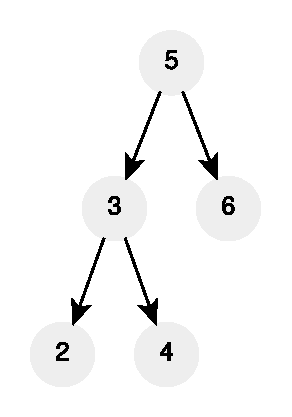
\includegraphics[width=\textwidth]{sources/remove_all_occurrences_unsorted_array_inplace/images/example1}
%	\caption[Sample short cpation]{Sample Caption}.
%	\label{fig:remove_all_occurrences_unsorted_array_inplace:example1}
%\end{figure}

\chapter{Remove all occurrences}
\label{ch:remove_all_occurrences_unsorted_array_inplace}
\section*{Introduction}
The problem described in this chapter asks you to implement a common operations: 
removes all elements satisfying specific criteria from a collection.
This problem shares  lot of similarities with the one described in Chapter \ref{ch:remove_duplicated_sorted_array_inplace}
and as a consequence they also share the same solution approach. 

There are many version of this problem. The most common is the one where the collection is a simple array of vector of integers
and you are ask to remove all the element equal to a given integer.
However we will discuss a more general version of this problem where the collection is of a generic type \inline{T}
and the criteria is given in the form of a unary function returning a boolean.

\section{Problem statement}
\begin{exercise}
\label{example:remove_all_occurrences_unsorted_array_inplace:exercice1}
Write a function that given a collection $I$ of elements of type
 \inline{T} and a predicate function $p$ having the following signature
 \inline{bool(const T&)} rearranges $I$ such that
 all the $k$ elements satisfying $p$  in $I$ are moved to the front of $I$.
 The function returns $k$.
 The relative order of the elements  satisfying $p$ should be preserved. 
 If the element at index $n$ and $m$ satisfy the predicate $p$  and $I_n$ comes before $I_m$ then
 when the function returns $I_n$ still comes before $I_m$.
 
	%example1
	\begin{example}
		\label{example:remove_all_occurrences_unsorted_array_inplace:example1}
		\hfill \\
		Given $I = \{[4, 1, 1, 2, 1, 3]\}$ and $p$ is a function returning true if its input element is 
		even, the function returns $4$ and the $4$ elements of $I$ are $\{1,1,1,3\}$. 
		
	\end{example}

	%example2
	\begin{example}
		\label{example:remove_all_occurrences_unsorted_array_inplace:example2}
		\hfill \
		
	\end{example}

	\begin{example}
		\hfill \
	
	\label{ex:remove_all_occurrences_unsorted_array_inplace:example3}
	\end{example}

	\begin{example}
		\hfill \

	\label{ex:remove_all_occurrences_unsorted_array_inplace:example4}	
	\end{example}
\end{exercise}

\section{Clarification Questions}

\begin{QandA}
	\item 
	\begin{answered}
		\textit{}
	\end{answered}
	
\end{QandA}

\section{Discussion}
\label{remove_all_occurrences_unsorted_array_inplace:sec:discussion}


\subsection{Brute-force}
\label{remove_all_occurrences_unsorted_array_inplace:sec:bruteforce}

\begin{minipage}{\linewidth}
	\lstinputlisting[language=c++, caption={Sample Caption},label=list:remove_all_occurrences_unsorted_array_inplace]{sources/remove_all_occurrences_unsorted_array_inplace/remove_all_occurrences_unsorted_array_inplace_solution1.cpp}
\end{minipage}

